\subsection{Tipo de observaciones}
La siguiente tarea a realizar era decidir que tipo de obsevaciones extraeriamos del entorno. Tal y como habiamos explicado en el apartado de Definición de conceptos, los agentes necesitan conocer el estado del entorno para poder aprender y tomar sus acciones. Para ello es necesario obtener una observación del juego. 

Existen dos principales formas de obtener el estado del juego: Serializando alguna clase que contenga los pricipales elementos del juego o simplemente capturar la imagen producida por el videojuego. La primera alternativa se suele usar en entornos más simples donde los elementos importantes para entrenar son pocos y facilmente serializables. Un ejemplo de este tipo de entornos puede ser el entorno Level-Based Foraging visto en el apartado Estado del arte. En este entorno simplemente se pasa una cuadricula con los elementos que hay en cada una de ellas. Podemos ver la representación del entorno en la figura \ref {fig:foraging-2}.

\begin{figure}[h]
    \centering
    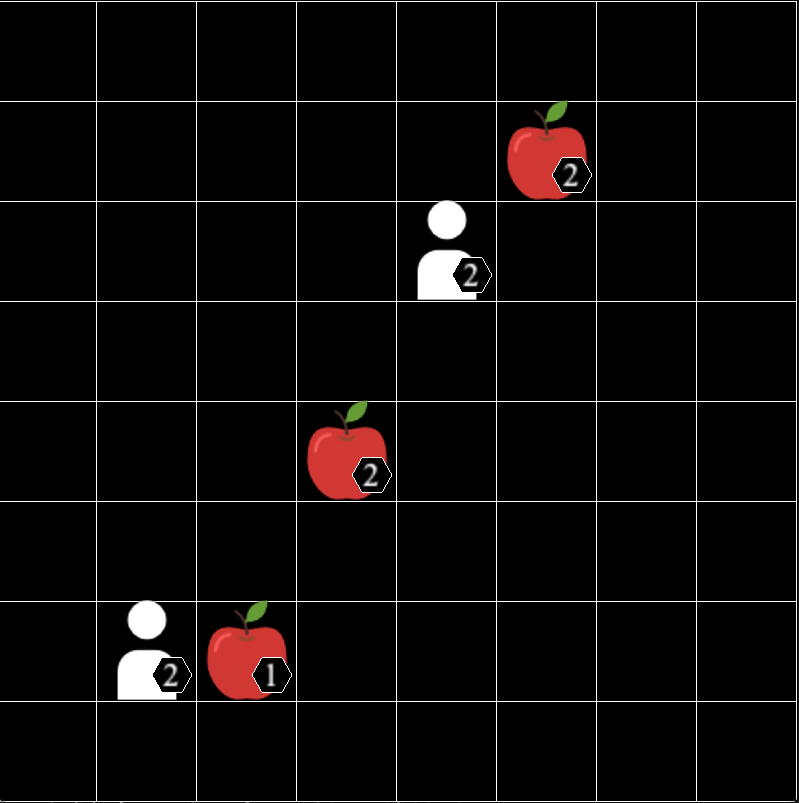
\includegraphics[width=0.3\textwidth]{img/level-base.png}
    \caption{Entorno gráfico de Level-Based Foraging \cite {env-list}}
    \label{fig:foraging-2}
\end{figure}

La segunda alternativa suele ser usada en entornos más complejos donde serializar todos los elementos es realmente complejo. Un ejemplo que utiliza esta alternativa es el entorno MALMÖ.

Nuestro entorno no es lo suficientemente simple para poder usar la primera opcion. Esto se debe los elementos importantes para el entrenamiento de un agente en nuestro entorno son muchos, muy variados y dificilmente serializables. Tomemos por ejemplo la figura \ref {fig:observartion} que forma parte de uno de los primeros niveles del mapa. 

\begin{figure}[h]
    \centering
    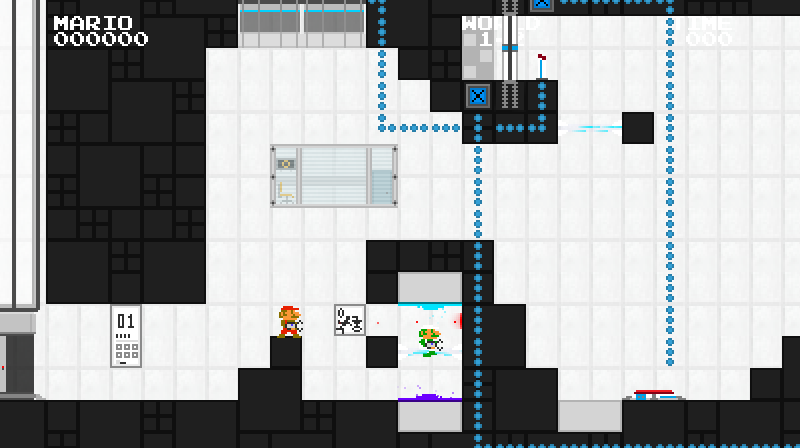
\includegraphics[width=0.9\textwidth]{img/BCTI_observation.png}
    \caption{Nivel del mapa Bowser Cooperative Testing Initiative \cite {mari0-mapa}}
    \label{fig:observartion}
\end{figure}

Esta sería la lista de elementos que deberíamos serializar para el entorno en caso de usar la primera alternativa:

\begin{itemize}
    \item Todos los bloques donde los jugadores pueden golpearse, incluyendo el techo del mapa. Esto es asi ya que gracias a los portales estos bloques pueden ser obstaculos o tener un papel relevante en el nivel.
    \item La posicion de los jugadores.
    \item La posicion de botones, pulsadores, palancas de salto, dispensadores de gel, puertas y dispensadores de cajas. Y además incluir la relación de que elementos accionan cada boton, pulsador etc.
    \item Todos los bloques donde los jugadores pueden colocar portales.
    \item Lasers azules, lasers rojos y lasers de destruccion de portales.
    \item Partes acuaticas o de acido.
    \item Enemigos y elementos dañinos.
\end{itemize}

Serializar esto es una tarea complicada y más aun teniendo en cuenta que los modulos del sistema no estan diseñados para esto. Si el juego se hubiera diseñado con la idea de pasar todos estos elementos a otro programa, esta sería una opcion viable. Pero en nuestro caso, esta opcion requeriría reconstuir practicamente todo el juego, algo impracticable. De modo que la unica opcion que queda es capturar las imagenes producidas por el videojuego y enviarlas a los agentes. Para esto, se decidio utilizar la resolución base del videojuego (600 x 800) y obtener sus imagenes en formato RGB. Por lo tanto, el tamaño de la observación sería 800 * 600 * 3 * 255.